\documentclass[12pt]{article}
\usepackage[letterpaper,top=2cm,bottom=2cm,left=3cm,right=3cm,marginparwidth=1.75cm]{geometry}
\usepackage[spanish]{babel}
\usepackage[utf8]{inputenc}
\usepackage[T1]{fontenc}
\usepackage{fancyhdr}
\usepackage{bm}
\usepackage{mathtools}
\usepackage{graphicx}
\usepackage{bbold}
\usepackage{yhmath} % pour pouvoir obtenir le symbole des ouverts avec une parenthèse
\usepackage{amsmath}    % les symboles les plus fréquents
\usepackage{amssymb}    % des symboles
%deux packages qui étaient dans le truc de Nou
\usepackage{enumitem} % pour les listes
\usepackage{hyperref} %hyperliens

\usepackage{theorem}
\newtheorem{theorem}{Teorema}
\newtheorem{lemma}{Lema}
\newtheorem{observation}{Observaci\'on}
\newtheorem{proof}{Demostraci\'on}
\newtheorem{proposition}{Proposici\'on}
\newtheorem{definition}{Definici\'on}
\newtheorem{corollary}{Corolario}
\DeclareMathOperator\supp{supp } %pour faire des jolis supports

%il suffira de renommer 3 commandes par celles utilisées pour th, lemme, preuve si on veut changer le style des démonstrations notamment. package amsth + \theoremstyle ?


%environnement pour les démo sans compteur et en écriture normale :
\renewenvironment{proof}{%

\vspace{0.5cm}

  \noindent \textbf{Demostraci\'on :}
}{%

  ~\hfill{$\Box$}
}




\newcommand{\E}{\mathrm{E}}
\newcommand{\N}{\mathbb{N}}
\newcommand{\C}{\mathbb{C}}
\newcommand{\Var}{\mathrm{Var}}
\newcommand{\subg}{\mathrm{SubG}}
\newcommand{\R}{\mathbb{R}}
\newcommand{\pp}{\mathbb{P}}

\begin{document}

\section{NURBS}

\subsection{Pesos para circunferencias}

intersection of the tangent lines passing through the other two points (now we see why this
technique only works for arcs of less than 180◦). Its weight, w2, is the cosine of half of the
angle subtended by the arc. That is, if $\angle B1CB3 = \theta$, where C is the center of the circle, then
w2 =  $cos(\theta /2) $.

\begin{figure}[h]
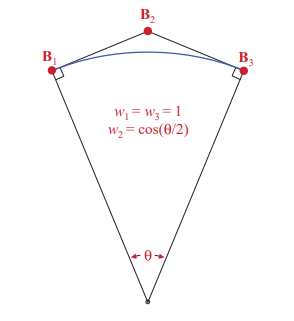
\includegraphics[width=5cm]{angulo.png}
\centering
\end{figure}

\section{Isogeometric analysis}

\subsection{Problema clasico}
\begin{figure}[h]
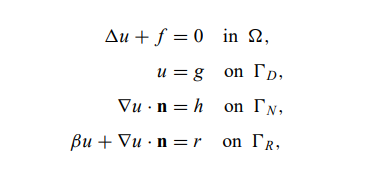
\includegraphics[width=6cm]{problema_clasico.png}
\centering
\end{figure}
\subsection{Formulación debil}
\begin{figure}[h]
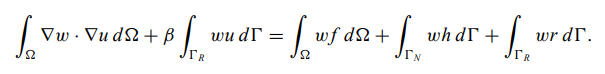
\includegraphics[width=9cm]{formulacion_debil.png}
\centering
\end{figure}
\subsection{Forma bilineal/ lineal}
\begin{align*}
  a(w,u)=L(w), &\\
  \text{Donde: }& \\
  &a(w,u) = \int_{\Omega} \nabla w \cdot \nabla u  d\Omega + \beta \int_{	\Gamma_R} wu d\Gamma,\\
  &L(w) = \int_{\Omega} \nabla w f  d\Omega + \int_{	\Gamma_N} wh d\Gamma+ \int_{	\Gamma_R} wr d\Gamma.\\
\end{align*}
\subsection{Discretización}
\begin{figure}[h]
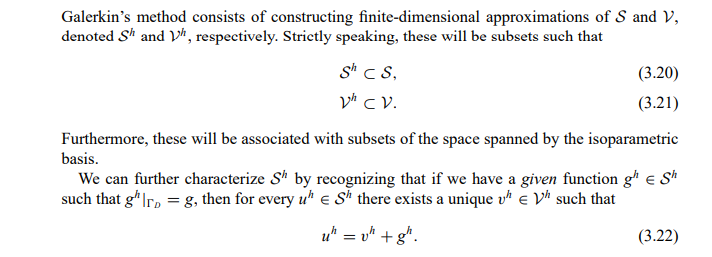
\includegraphics[width=15cm]{Discretizacion.png}
\centering
\end{figure}
\subsection{Forma bilineal/ lineal discretas}
\begin{equation*}
  a(w^h,u^h)=L(w^h) \implies a(w^h,v^h)=L(w^h)-a(w^h,g^h)  
\end{equation*}

\end{document}

